\documentclass{article}
\usepackage{tabularx}
\usepackage{amsmath}
\usepackage{graphicx}
\usepackage[top = 2cm, bottom = 2cm, right = 2cm, left = 2cm]{geometry}
\usepackage{cite}
\usepackage[final]{hyperref}
\usepackage{listings}
\hypersetup{
	colorlinks=true,
	linkcolor=blue,
	citecolor=blue,
	filecolor=magenta,
	urlcolor=blue         
}

\begin{document}

\title{Practicle 4\\Raytracer - Sphere}
\date{23/01/19}
\maketitle

\begin{abstract}
	The last practicals focused on sending rays. Here, we will see how to grab information from a virtual scene and display it.
\end{abstract}

\section{Intersect a sphere}
To compute the intersection between a ray and a sphere we'll use an analytic method. The implicit function of a sphere is: $x^2+y^2+z^2 = R^2$ with $P(x, y, z)$ a point in the surface sphere centered in the origin with a rayon of R. We want only points on the ray so we just need to replace $P$ by the ray equation : \\
$|O+Dt|^2 = R^2,$\\
$O^2 + 2DtO + (Dt)^2 = R^2,$\\
$O^2 + D^2t^2 + 2ODt = R^2,$\\
$O^2 + D^2t^2 + 2ODt - R^2 = 0,$\\
We want to find the $t$ value for the ray.\\
$ D^2t^2 + 2ODt + O^2 - R^2 = 0,$\\
with $a = D^2$, $b = 2OD$ and $c = O^2 - R^2$ we get a quadratic function ($f(t) = at^2+bt+c$)\\
If we want to move the sphere we just need to subtract the center $C$ to $P$ and $O$. The equation becomes: $|(O-C)+Dt|^2 = R^2;$
We get $a = D^2$, $b = 2(O-C)D$ and $c = (O-C)^2 - R^2$. Because the product for vector is the dot product and D is normalized, $a=1$\\
Remember that quadratic function can be solved in this way: $t_i = \frac{-b\pm \sqrt{b^2-4ac}}{2a}$

\section{C++ implementation}
Create a Sphere class into the device side for storing the center and the radius information. Create now the intersect function: 
\begin{lstlisting}
	__device__ bool Sphere::intersect(const Ray& ray, float& t) {
		float t0, t1;
		Vector3GPU OC = ray.getOrigin() - center_;
		float b = 2.f*dot(oc, ray.getDirection());
		float c = dot(oc, oc) - radius_*radius_;
		// ...
	}
\end{lstlisting}
if the discriminant is negative you just have to return false and don't modify the final image buffer. If there is a collision, just return the red color. For information the smallest value of t is the nearest intersection point.
\begin{figure}[h]
	\centering
	
\includegraphics[scale=0.6]{figures/intersect.png}
	\caption{Intersection ray sphere}
\end{figure}

\newpage
\section{Compute and show normal information}
When you intersect the sphere you can compute some geometry information like the normal of the point from the intersection point.
\begin{figure}[h]
	\centering
	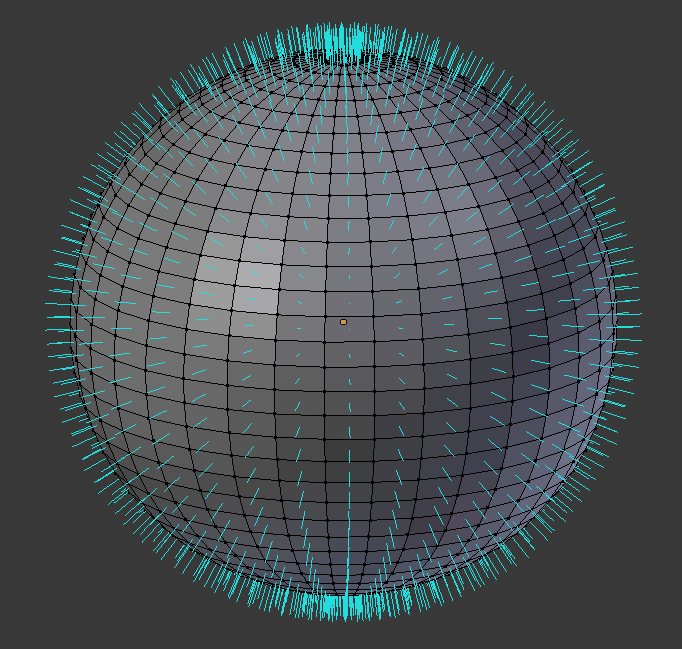
\includegraphics[scale=0.4]{figures/normal.png}
	\caption{Normal of a sphere}
\end{figure}
\begin{lstlisting}
	Vector3 intersection = ray.getOrigin()+ray.getDirection()*t;
	Vector3 normal = (intersection-world[wid].center_);
\end{lstlisting}

To be sure our normal is correctly computed we can show them on the sphere. We just have to be careful because normal are between (-1, -1, -1) and (1, 1, 1). So we just have to multiply the normal by 0.5 and add the vector (0.5, 0.5, 0.5) to match the $[0, 1]^3$ range.
\begin{figure}[h]
	\centering
	
\includegraphics[scale=0.6]{figures/intersectnormal.png}
	\caption{Intersection ray sphere}
\end{figure}
\newpage
\section{A world of spheres}
To avoid the creation of the world inside each kernel we can generate it one on the host side. Add the keyword \_\_host\_\_ to the constructor of the Sphere class and create a buffer of spheres. 
\begin{lstlisting}
std::vector<Sphere> spheres;
world.push_back(Sphere(Vector3(0.f, 0.f, -3.f), 0.5f));
world.push_back(Sphere(Vector3(0.f, -100.5f, -3.f), 100.f));
Sphere* spheresGPU;
cudaMalloc(&spheresGPU, sizeof(Sphere)*spheres.size());
cudaMemcpy(spheresGPU, &spheres[0], sizeof(Sphere)*spheres.size(), cudaMemcpyHostToDevice);
\end{lstlisting}
\begin{figure}[h]
	\centering
	
\includegraphics[scale=0.45]{figures/intersectnormaltwosphere.png}
	\caption{Intersection ray two spheres}
\end{figure}

For advenced groups, you can take a look in other intersection at this address: http://iquilezles.org/www/articles/intersectors/intersectors.htm

\newpage
\section{CUDA errors}
Each CUDA function return error value. We can store it in a cudaError\_t.
\begin{lstlisting}
	cudaError_t err = cudaMalloc(...);
	if (err != cudaSuccess) {
		std::cout<<cudaGetErrorString(err);
	}
\end{lstlisting}
The kernel computation don't return value. So if there is an error in the kernel we have to wait the end of the kernel execution and synchronize the device with the host and grab the last error.\\
Most of the time, when we compute heavy algorithm we get some error about kernel configuration. Commun errors are:
\begin{itemize}
	\item Too Many Resources Requested for Launch (That mean each thread need more registe that the SM can provide. Reducing the number of thread per block solve this error)
	\item an illegal memory access was encountered. You may read values outside your buffers or you stack pointer (GPU threads are designed to be short process. If you use recursive function you may saturate one of your callstack and get this error. If you really need to call a lot of function, you can increase the size of your callstack using cudaDeviceSetLimit)
\end{itemize}
\begin{lstlisting}
	cudaError_t err = cudaGetLastError();
	if (err != cudaSuccess) {
		std::cout<<cudaGetErrorString(err);
	}
\end{lstlisting}

\end{document}